% public transport map
\DeclareNewLayer[background,%
  width=105mm,%
  height=148mm,%
  hoffset=10mm,%
  voffset=10mm,%
  contents={%
    %TODO correct size
    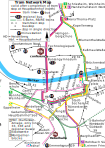
\includegraphics[]{images-print/public_transport.pdf}%
  }%
]{publictransport}
\newpairofpagestyles[]{page-public-transport}{}
\AddLayersAtBeginOfPageStyle{page-public-transport}{publictransport}
\AddLayersAtBeginOfPageStyle{page-public-transport}{cropmarksplain}

% city map
\definecolor{tram}{cmyk}{0 0 0 0.62}
\DeclareNewLayer[background,%
  width=115mm,%
  height=158mm,%
  hoffset=5mm,%
  voffset=5mm,%
  contents={%
    \begin{tikzpicture}[x=1mm, y=1mm]%
      % map image
      \draw (0,0) node [inner sep=0mm, anchor=south west] {%
        \includegraphics[width=115mm]{images-print/heidelberg-map-left.png}%
      };%
      % box for map key
      \fill [white] (0,32) rectangle (52,0);%
      % map key text
      \draw (8,8) node [anchor=south west, align=left] {%
        \begin{minipage}{47mm}%
          \small
          1 Conference \hspace{1em}
          2 Botanic Garden \hspace{1em}\linebreak
          3 Tram Stop Hbf (since 2019-09-11) \hspace{1em}
          4 HebelHalle\hspace{1em}
          5 Bridge closed \hspace{1em}\linebreak
          6 Philosophenweg \hspace{1em}\linebreak
          7 Old Bridge and Bridge Monkey \hspace{1em}\linebreak
          8 Marstall \hspace{1em}
          9 Castle
        \end{minipage}%
      };
      % tram line
      \draw [line width=0.33mm, color=tram] (64.95,48.95) -- (68.97,47.38) .. controls (70.63,46.87) and (72.80,45.17) .. (75.64,45.57) -- (89.85,49.39);
      \draw [line width=0.30mm, color=tram] (64.98,48.55) -- (68.92,46.98) .. controls (70.58,46.47) and (72.75,44.97) .. (75.64,45.57) -- (89.85,49.39);
      % circles with numbers
      \node (1) at (68.74,47.41) [] {}; % Hbf Nord
      \node (1label) at (1) [fill=white, draw=black, inner sep=0.3mm, circle] {\small 3}; % Hbf Nord (label)
      \node (2) at (90.6, 13.0) [] {}; % Hebelbrücke
      \node (2label) at (2) [fill=white, draw=black, inner sep=0.3mm, circle] {\small 5};
      \node (3) at (60.6, 110.5) [] {}; % Chemie-Hörsaalgebäude
      \node (3label) at (3) [fill=white, draw=black, inner sep=0.3mm, circle] {\small 1}; % Chemie-Hörsaalgebäude
      \node (4) at (78.31, 9.02) [] {}; % Hebelhalle
      \node (4label) at (4) [fill=white, draw=black, inner sep=0.3mm, circle] {\small 4};
      \node (5) at (43.3, 93.8) [] {}; % Botanischer Garten
      \node (5label) at (5) [fill=white, draw=black, inner sep=0.3mm, circle] {\small 2}; % Botanischer Garten
    \end{tikzpicture}%
  }%
]{citymapleft}
\newpairofpagestyles[]{page-citymap-left}{}
\AddLayersAtBeginOfPageStyle{page-citymap-left}{citymapleft}
\AddLayersAtBeginOfPageStyle{page-citymap-left}{cropmarksplain}
\DeclareNewLayer[background,%
  width=115mm,%
  height=158mm,%
  hoffset=5mm,%
  voffset=5mm,%
  contents={%
    \begin{tikzpicture}[x=1mm, y=1mm]%
      % node for extend
      % map image
      \draw (0,0) node [inner sep=0mm, anchor=south west] {%
        \includegraphics[width=115mm]{images-print/heidelberg-map-right.png}%
      };%
      % circles with numbers
      \node (6) at (55.4, 103.3) [] {}; % Philosophenweg
      \node (6label) at (6) [fill=white, draw=black, inner sep=0.3mm, circle] {\small 6};
      \node (7) at (81.3, 74.9) [] {}; % castle
      \node (7label) at (7) [fill=white, draw=black, inner sep=0.3mm, circle] {\small 9};
      \node (8) at (62.9, 87.7) [] {}; % Old Bridge
      \node (8label) at (8) [fill=white, draw=black, inner sep=0.3mm, circle] {\small 7};
      \node (9) at (48.1, 84.46) [] {}; % Old Bridge
      \node (9label) at (9) [fill=white, draw=black, inner sep=0.3mm, circle] {\small 8};
    \end{tikzpicture}%
  }%
]{citymapright}
\newpairofpagestyles[]{page-citymap-right}{}
\AddLayersAtBeginOfPageStyle{page-citymap-right}{citymapright}
\AddLayersAtBeginOfPageStyle{page-citymap-right}{cropmarksplain}

% campus map
\DeclareNewLayer[background,%
  width=115mm,%
  height=158mm,%
  hoffset=5mm,%
  voffset=5mm,%
  contents={%
    %TODO correct size
    \includegraphics[]{images-print/campus.pdf}%
  }%
]{campus}
\newpairofpagestyles[]{page-campus}{}
\AddLayersAtBeginOfPageStyle{page-campus}{campus}
\AddLayersAtBeginOfPageStyle{page-campus}{cropmarksplain}
